\documentclass[12pt]{article}
\usepackage[a4paper, total={6.5in, 10in}]{geometry}

\usepackage{amsmath}
\usepackage{amssymb}
\usepackage{enumitem}
\usepackage{braket}
\usepackage{qcircuit}
\usepackage{graphicx}

\newcommand{\code}{CS-IS-2010-1}
\newcommand{\name}{Midsemester Project Report}
\newcommand{\me}{Santripta Sharma}

\newcommand{\prob}[1]{\mathbb{P}\left[#1\right]}

\newcommand{\kz}{\ket{0}}
\newcommand{\ko}{\ket{1}}
\newcommand{\kp}{\ket{\phi}}
\newcommand{\ks}{\ket{\psi}}
\newcommand{\kso}{\ket{\psi_1}}
\newcommand{\kst}{\ket{\psi_2}}


\newcommand{\rec}[1]{\frac{1}{#1}}

\newenvironment*{qparts}{\begin{enumerate}[label=(\alph*)]}{\end{enumerate}}

\title{\code: \name}
\author{\me}
\date{\today}

\markright{\code\hspace{0.5in}\name\hspace{0.5in}\me}

\parindent=0pt

\begin{document}
\maketitle
\hrule \bigskip

\section{Problem}
This project is concerned with building a tool for running inference over a given feed-forward neural network. In particular, we are interested in inferencing a network trained on the Iris Dataset, where the goal is to classify Iris flowers into one of three species --- setosa, verticolor, or virginica --- based on the following four features:
\begin{enumerate}
	\item Sepal length
	\item Sepal width
	\item Petal length
	\item Petal width
\end{enumerate}

Since we are only concerned with running the inference for a new row for this dataset, we train a classification model separately (for testing purposes) before runtime. At runtime, we restore the structure, weights, and biases of the model, and push the given feature vector through the model in order to arrive at the inferred output.

\section{Specification}
Formally, we are creating a tool which meets the following specification:\bigskip

\textbf{Inputs:} 
\begin{itemize}
	\item File containing saved model structure, weights, and biases (in some format)
	\item Batch of feature vectors to run the inference for (stdin)
\end{itemize}

\textbf{Outputs:}
For every vector in the input batch,
\begin{itemize}
	\item Most likely class for this observation (string)
	\item Activation values associated with each class at the output layer (vector)
\end{itemize}

\subsection{Project Architecture}
The project can broadly be divided into two modules, the training module \& the inference module. These operate independently from each other, with the only interface between them being the inference module taking the training module's output (model structure, weights, biases) as its input.

\newpage
\begin{figure}
	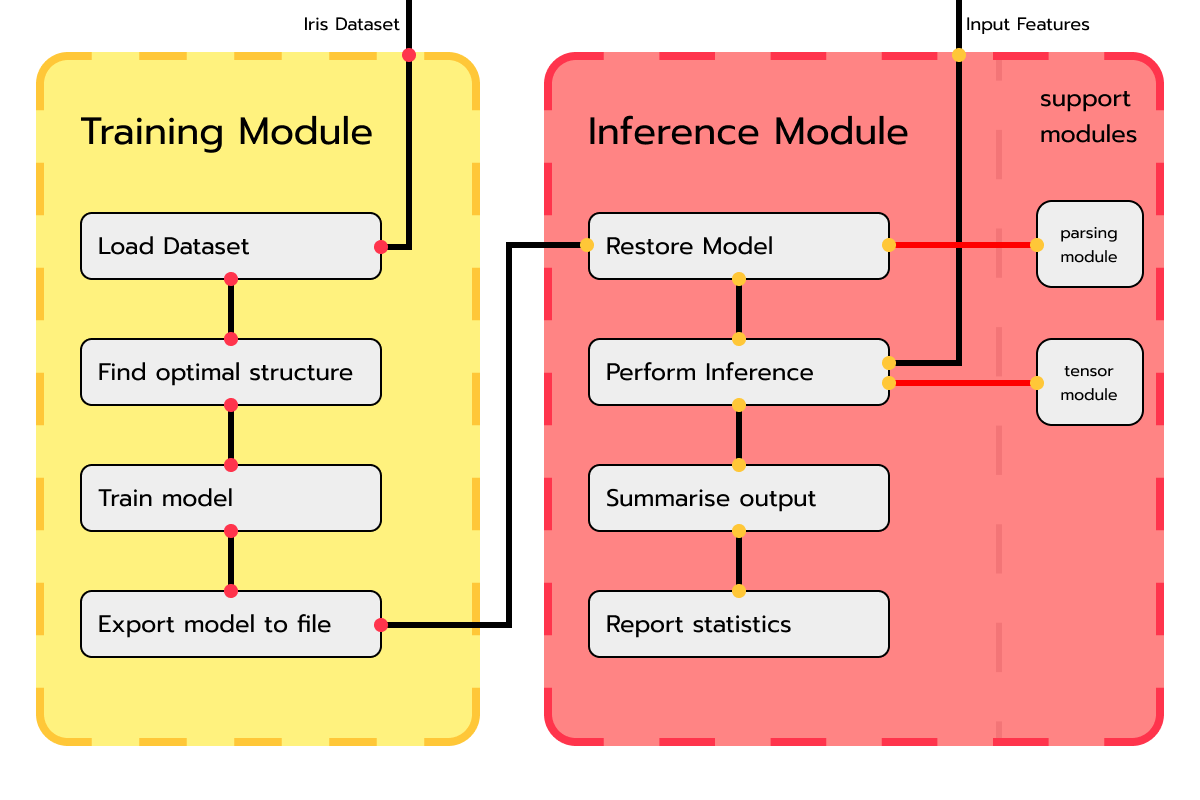
\includegraphics[width=0.85\pdfpagewidth]{../images/modules.png}
	\caption{a pictorial representation of the high-level architecture}
\end{figure}

Then, due to their decoupling, we can individually dissect each of the modules.

\subsubsection{Training Module}
The purpose of the training module is to provide us with a set of models we can use to test our inference module. As such, we don't strictly require a high performance model. However, we still perform some basic hyperparameter selection after loading the dataset in using a 5-fold cross validation approach to determine the shape of the network (number \& size of hidden layers).\bigskip

The model architecture used is a simple feedforward network. Using a grid search, we find the top 5 performing models, and also one poorly performing model, out of a generated set of possible shapes for the network.\bigskip

Finally, we write the networks' shapes, weights, and biases into a text file, which can then be used by the inference module to restore the model. In later versions of the project, the intention is to transition this into a binary file format, for higher time \& space efficiency at the restoration stage.

\subsubsection{Inference Module}
The inference module constitutes the bulk of the codebase. Its first task is to restore the model from the file exported by the training module. This utilises the parsing support module, which is simply the inverse operation of the export performed as the training module's final step.\bigskip

The model shape, and its parameters are loaded into a data structure which takes the form of a linked list of layers, where each layer stores its input shape, neuron count, and the weights \& biases matrices.\bigskip

Based on the user's input feature vectors, the inference is performed using simple matrix operations, which are supported by the tensor module. 

\subsection{Tooling}
\subsubsection{Training Module}
The training module is written in python, using numpy, pandas, and sklearn to perform the data processing \& model training/selection.\bigskip

\subsubsection{Inference Module}
Ok

\subsubsection{Testing}
Oker

\subsection{Test Plan}
\subsubsection{Unit Tests}
Real

\subsubsection{Integration Tests}
Realer

\subsubsection{End-to-End Tests}
Realest

\section{Prototype Details}
Greatest Prototype of all Time

\section{Plan for Completion}
Greatest Completion of all Time

\end{document}